\documentclass{article}

% This defines the title
\newcommand{\Title}{Semiconductor lab}

% This defines the course
\newcommand{\Course}{FYSC23}

% First author
\newcommand{\AuthorOne}{Fredrik Bergelv}

\newcommand{\EmailOne}{fredrik.bergelv@live.se}

% Second author
\newcommand{\AuthorTwo}{Max Eriksson}

\newcommand{\EmailTwo}{maxerikss@gmail.com}

% Information about supervisor
\newcommand{\SupervisorInfo}{}

% Is table of contents wanted?
\newcommand{\IncludeTab}{true} 

% Is bibliography wanted?
\newcommand{\IncludeBib}{true} 


\usepackage[utf8]{inputenc}
\usepackage[T1]{fontenc}
\usepackage[a4paper,margin=25mm,headsep=5mm,headheight=12pt]{geometry}
\frenchspacing
\usepackage{amsmath,amssymb,amsfonts,amsthm}  
\usepackage{hyperref} 
\hypersetup{
    colorlinks, 
    citecolor=black,
    filecolor=black, 
    linkcolor=black,
    urlcolor=black
}
\usepackage{setspace}
\usepackage{graphicx}
\usepackage{subcaption}
\usepackage[separate-uncertainty=true]{siunitx} 
\sisetup{
  range-phrase=--,
  detect-all,
  output-decimal-marker={.},
  range-units=single,
  per-mode=reciprocal, 
}
\usepackage{url}
\usepackage{verbatim}
\usepackage[toc,acronym]{glossaries}
\usepackage{booktabs} 
\usepackage{fancyhdr} 
\usepackage{lipsum}
\usepackage{lastpage} 
\usepackage{float} 
\usepackage{listings} 
\usepackage{comment} 
\usepackage{tcolorbox}
\usepackage{svg}


\setlength{\parindent}{0pt}
\setlength{\parskip}{2em}

\pagestyle{fancy}
\fancyhead[L]{\footnotesize \textsc{\AuthorOne \ \AuthorTwo}}
\fancyhead[R]{\footnotesize \textsc{\leftmark}}
\fancyfoot[R]{ \thepage}
\fancyfoot[C]{}
\bibliographystyle{unsrt}

% MY OWN PACKAGES


\newcommand{\abs}[1]{\left| #1 \right|}

\newcommand{\expectation}[1]{\left< #1 \right>}

\newcommand{\scalar}[2]{\left< #1 | #2 \right> }

\newcommand{\derivate}[2]{\frac{\partial #1}{\partial#2}}

\newcommand{\expscalar}[2]{\left< #1 \left| #2\right| #1 \right>}

\newcommand{\optscalar}[3]{\left< #1 \left| #2\right| #3 \right>}

\newcommand{\set}[1]{\left\{#1 \right\}}

\newcommand{\norm}[1]{\left\|\Vec{#1} \right\|}

\newcommand{\expect}[1]{\left\langle #1 \right\rangle}

\newcommand{\nuc}[2]{\text{${}^{#1}$#2}}

\newcommand{\uvec}[1]{\mathbf{\hat{#1}}}


\DeclareSIUnit\angstrom{\protect \text {Å}}

\DeclareSIUnit\atomicmassunit{u}

\newenvironment{question}
  {\begin{tcolorbox}[colframe=white!50!black, colback=white!10!white, title=Question] }
  {\end{tcolorbox}}           

\newenvironment{answer}
  {\begin{tcolorbox}[colframe=white!50!black, colback=white!10!white, title=Answer] }
  {\end{tcolorbox}}           





\usepackage{titlesec}
\titlespacing*{\section}{0pt}{4pt plus 2pt minus 2pt}{4pt plus 2pt minus 2pt}
\titlespacing*{\subsection}{0pt}{4pt plus 2pt minus 2pt}{4pt plus 2pt minus 2pt}

\begin{document}

\begin{titlepage}  

	\newcommand{\HRule}{\rule{\linewidth}{0.5mm}}
	
 \centering 	
 
	\textsc{\LARGE \Course}\\[2cm] 
 
	\HRule\\[1.0cm]
 
	{\huge\bfseries \Title }\\[0.4cm] 
 
	\HRule\\[1.5cm]
 
	\begin{minipage}[t]{0.5\textwidth}
	\begin{center}
 
		\large
   
		\textit{Authors}\\
   
		\AuthorOne \\
        \AuthorTwo
            
        \href{mailto:\EmailOne}{\texttt{\EmailOne}} \\
            
        \href{mailto:\EmailTwo}{\texttt{\EmailTwo}}
            
        \vspace{5mm}
                
        \SupervisorInfo
                
	\end{center}
	\end{minipage}

	\vfill\vfill\vfill\vfill
 
   
\includegraphics[width=0.4\textwidth]{Figures/Lund logo.png}
    \\ \textsc{\LARGE {LUND UNIVERSITY}}
    
	\vfill\vfill\vfill 
 
    \today
        
	\vfill 
 
\end{titlepage}


\section*{Abstract}

\newpage

\ifthenelse{\equal{\IncludeTab}{true}}{\pagestyle{empty}
\tableofcontents
\newpage
\setcounter{page}{1}
\pagestyle{fancy}}{}

\section{Introduction}
\section{Experiment}
\subsection{Part 1}



Wavelength white LED: 454.17 nm 




\begin{table}[H]
    \centering
    \begin{tabular}{@{}lllll@{}}
        \toprule
        Mesurment & V\textsubscript{in} (V) & V\textsubscript{across} (V) & I\textsubscript{circuit} (mA) & Intensity (counts) \\ \midrule
        1         & 1                       & 1.14                        & 0.0                           & 5.00               \\
        2         & 1.8                     & 1.96                        & 0.0                           & 8.00               \\
        3         & 2.2                     & 2.41                        & 0.00                          & 4.70               \\
        4         & 2.5                     & 2.56                        & 0.36                          & 590.30             \\
        5         & 2.9                     & 2.66                        & 3.11                          & 4377.70            \\
        6         & 3.3                     & 2.72                        & 6.21                          & 7979.50            \\
        7         & 3.7                     & 2.76                        & 9.24                          & 10846.90           \\
        8         & 4.4                     & 2.84                        & 15.24                         & 16080.10           \\
        9         & 5.3                     & 2.93                        & 24.5                          & 21958.10           \\
        10        & 6.5                     & 3.02                        & 35.2                          & 27642.20           \\
        11        & 7.3                     & 3.08                        & 42.6                          & 30184.80           \\
        12        & 8.3                     & 3.15                        & 52.0                          & 33590.00           \\
        13        & 9.1                     & 3.20                        & 59.0                          & 36153.70           \\ \bottomrule
        \end{tabular}
    \caption{tab:part1}
    \end{table}


    
\section{Result}
\subsection{Part 1}
In the first part the peak which was measured from the white diode was located at \SI{454.17}{\nano\m}. Using the data obtained from the measurements \autoref{fig:part1} was obtained. From the linear fit in \autoref{fig:a} one can see that that the linear fit intersects the x-axis at $V_\text{in}=\SI{2.7}{\V}$. This means that a voltage under this value would yield no current output, which can be seen in the figure. Thus, one can conclude that the forward bias is $V_\text{in}=\SI{2.7}{\V}$. 

\begin{figure}[H]
    \centering
    \subfloat[This plot displays the itensity of the LED over the current in the circuit. ]{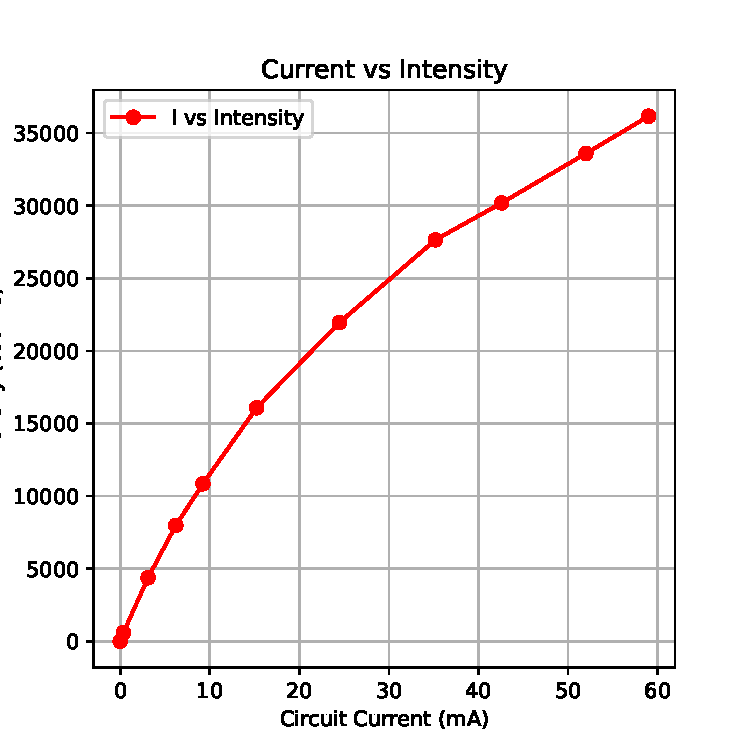
\includegraphics[width=0.49\textwidth]{Figures/part1(b).pdf} \label{fig:a}}
    \hfill
    \subfloat[This plot displays the itensity of the LED over the voltage across the LED in the circuit.]{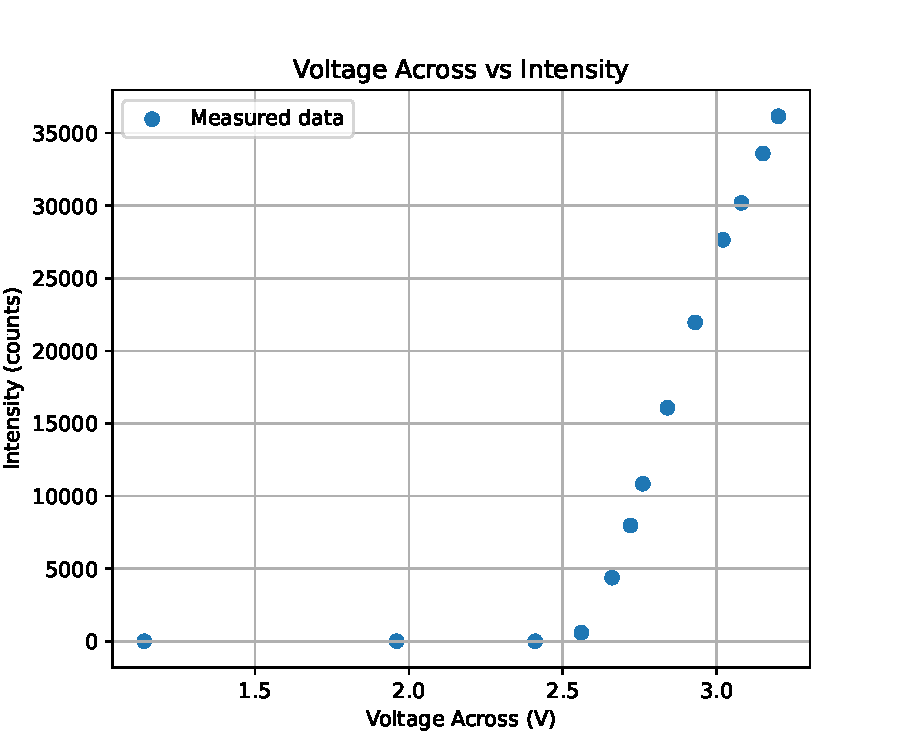
\includegraphics[width=0.49\textwidth]{Figures/part1(c).pdf} \label{fig:b}}
    
    \vspace{0.5cm}
    
    \subfloat[This plot displays the current in the circuit over the voltage from DC-source. A linear fit was used for the non-zero measurements, since this fit would be used to calculate the forward bias. ]{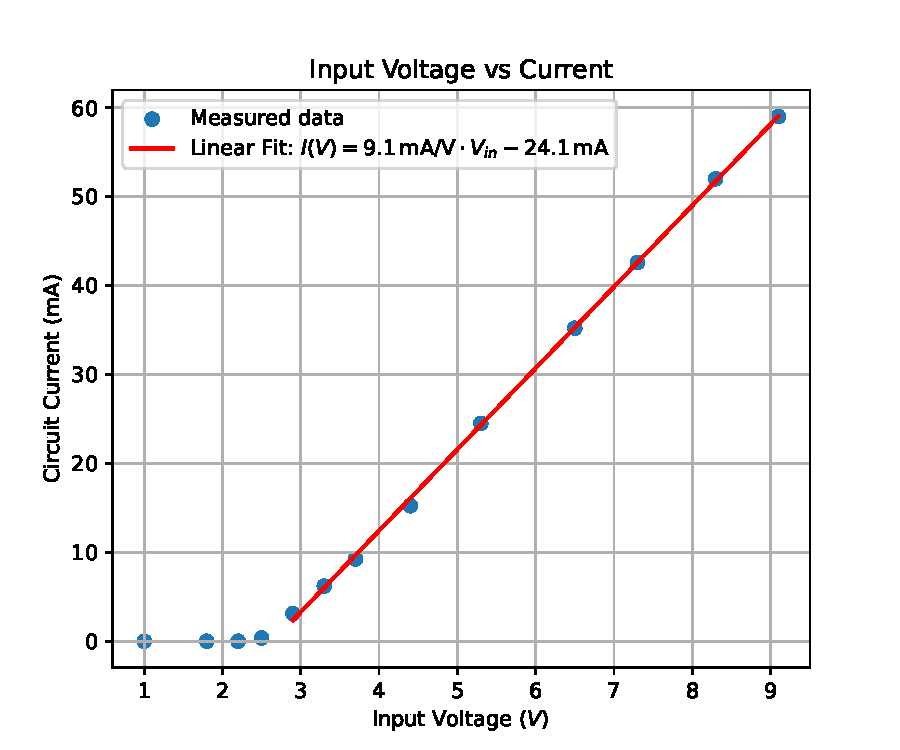
\includegraphics[width=0.49\textwidth]{Figures/part1(a).pdf} \label{fig:c}}

    \caption{Plots of the measurements.}
    \label{fig:part1}
\end{figure}




\subsection{Part 2}
The measurements from the circuit before was combined with the measurements from the program, as seen in \autoref{fig:part2}, in \autoref{tab:part2}. Notably the wavelength of the peak shifted, and the intensity increased when the diode was submerged in liquid nitrogen.

\begin{table}[H]
    \centering
    \caption{This table shows the measurements.}
    \begin{tabular}{@{}llllll@{}}
    \toprule
    Measurement      & V\textsubscript{in} (V) & V\textsubscript{LED} (V) & I\textsubscript{circuit} (mA) & $\lambda_\text{peak}$ (nm) & Intensity (counts) \\ \midrule
    Room temperature & 5.0& 2.06& 30.8& 596.70& 2663.70\\
    Liquid nitrogen  & 5.0& 4.44                     & 7.7& 569.69& 10757.70\\ \bottomrule
    \end{tabular}
    \label{tab:part2}
    \end{table}


\begin{figure}[H]
    \centering
    \subfloat[This was the output from the program at room temperature.]{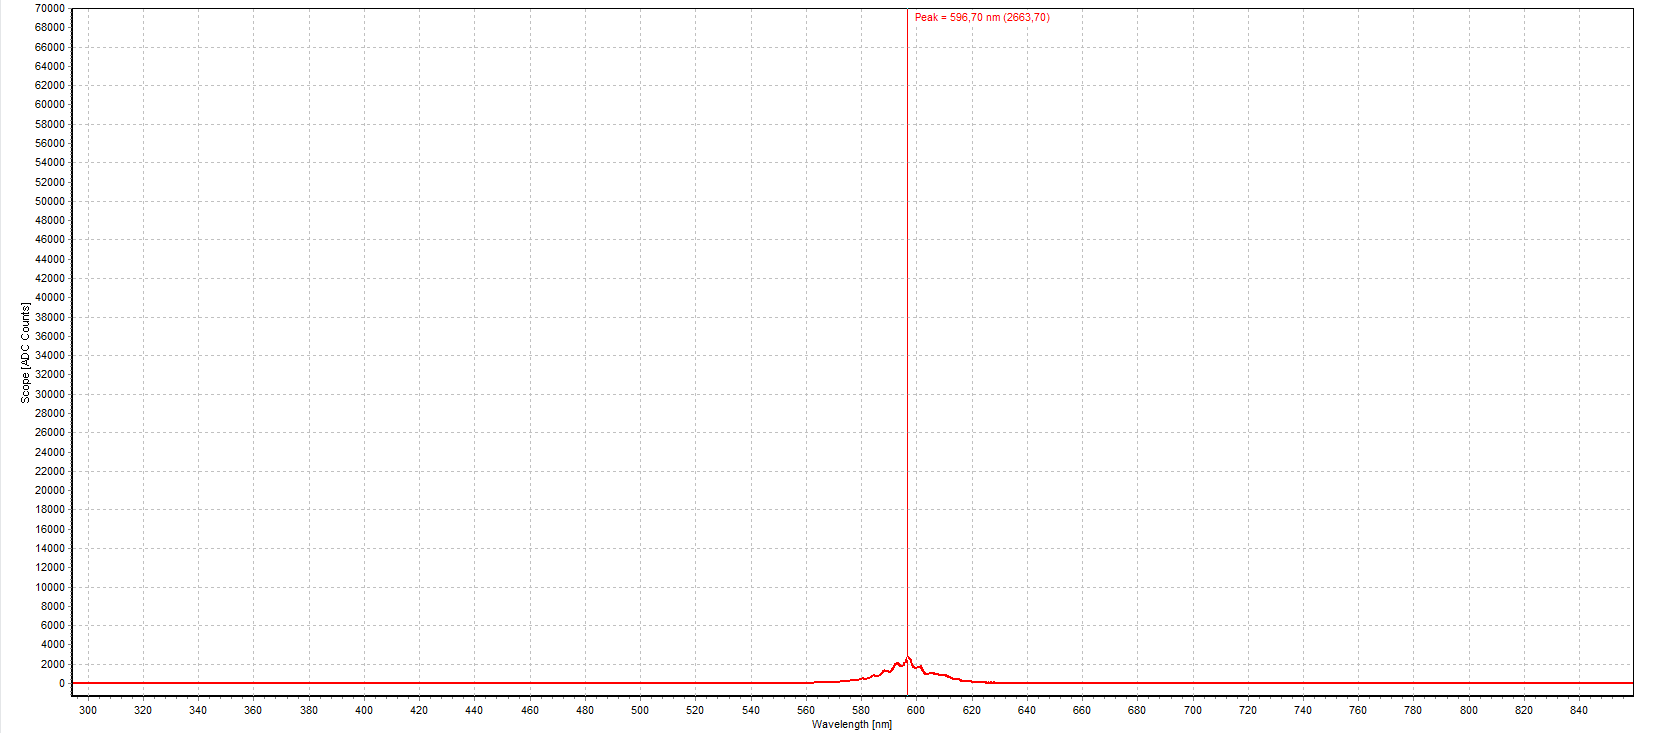
\includegraphics[width=0.5\textwidth]{Figures/Part2_before.png} \label{fig:before}}
    \hfill
    \subfloat[This was the output from the program when submerged in liquid nitrogen.]{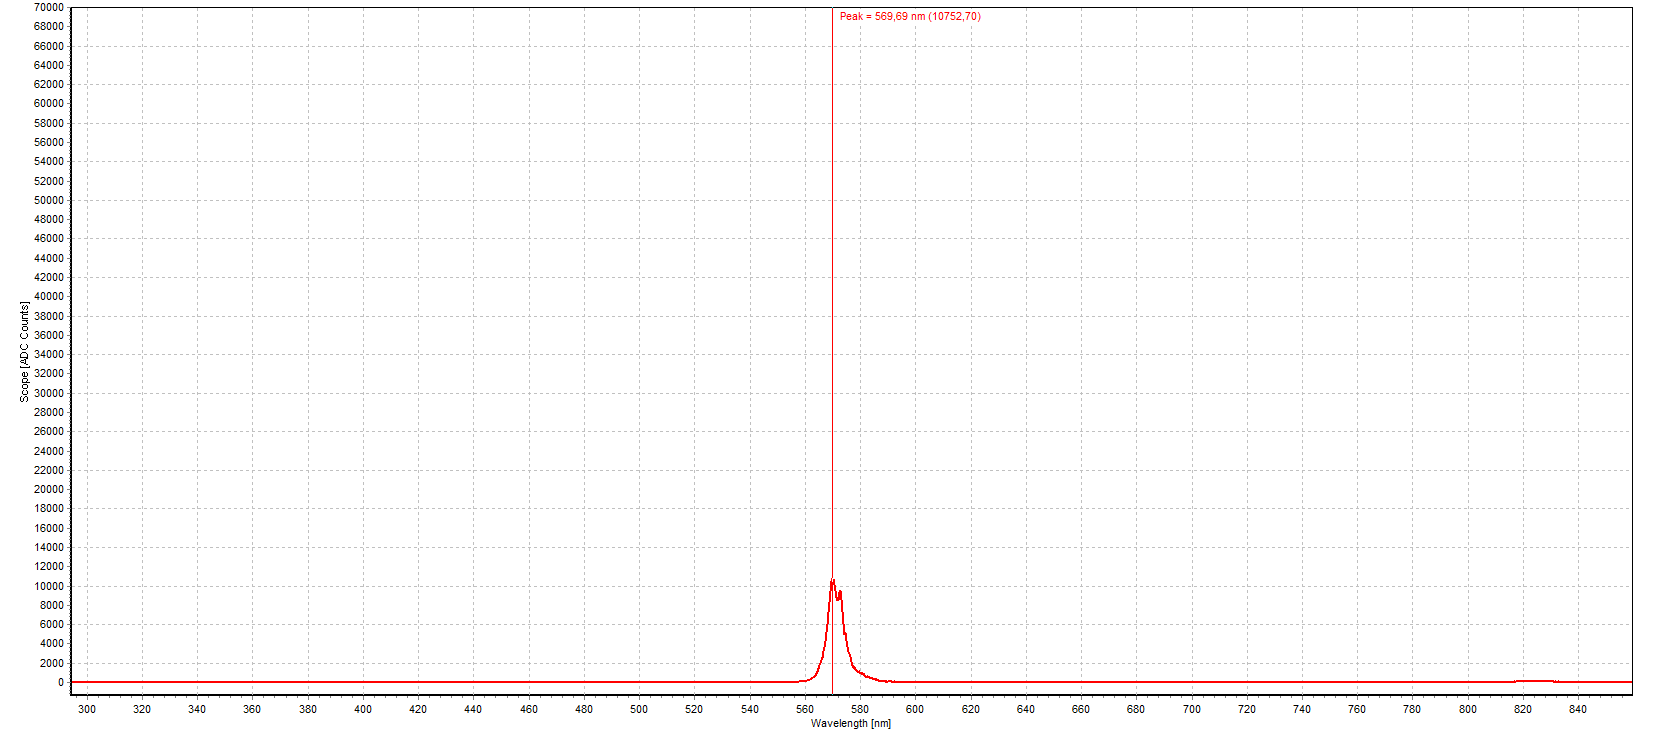
\includegraphics[width=0.5\textwidth]{Figures/Part2_after.png} \label{fig:after}}
    \caption{This figure display the output from AvaSoft at the different measurements.}
    \label{fig:part2}
\end{figure}




\subsection{Part 3}
The result from the different diode constellations as detectors and emitters can be seen in \autoref{tab:part3}. The table shows that shorter wavelength diodes can excite longer wavelength diodes, but not the other way around.

\begin{table}[H]
    \centering
    \caption{This table displays which combinations of detectors and emitters yielded an voltage output from the diode in the smaller circuit.}
    \begin{tabular}{@{}llll@{}}
    \toprule
    Detector/Emitter & Red    & Green     & Blue      \\ \midrule
    Red              & Output & No output & No output \\
    Green            & Output & Output    & No output \\
    Blue             & Output & Output    & Output    \\ \bottomrule
    \end{tabular}
    \label{tab:part3}
\end{table}
\section{Discussion}
\subsection{Part 1}
The emitted light has two main peaks. One peak was in the blue part of the spectrum while the other, broader peak was at the yellow part of the spectrum. This combination appears white to our eyes. The reason for the yellow peak is that the inside of the LED is coated with phosphor which is excited by the LED and then re-emit light in the yellow part of the spectrum.

After the threshold voltage is reached the current increases linearly with the voltage. The reason is that the amount of electron-hole pairs created is proportional to the energy deposited by the voltage. The voltage need to be applied in the forward direction to shin because there is no diffusion current in the reverse direction, and it is this current that recombines to emit light.

The intensity of the light increases with increasing current and voltage, which is expected since this increases the amount of electron and thus the rate of recombination. More recombination means more light Different coloured LEDs have different bandgaps and the threshold voltage will therefore be different. For white LEDs a blue or preferably violet is preferred since this excited the phosphor and the resulting light is white.

\subsection{Part 2}
The current drops when the sample was dropped into liquid nitrogen, which is due to the fact that the resistance is correlated with the temperature. Thus a much lower temperature gave a lower resistance, and thus a lower current. The light emission intensity increased when submerged. This is due to low temperature results in fewer phonons and thus less phonon scattering. Thus a low temperature means more electron- hole recombination, and thus more light emission. 

The change in wavelength of the LED corresponds to the low temperature implying a freeze out of the LED. This means that the donors/ acceptors does not have enough energy to get ionized and no doping occurs. Thus the band gap is increased, implying a lower wavelength of the emitted photons. This freeze out phenomenon should effect all doped materials. 


\subsection{Part 3}
For a diode used as a solar cell the bandgap should be small enough to absorb as much light as possible from the sun's spectrum, but large enough to extract energy. Too small of a bandgap will be easily excited but after thermalization of the election most of the energy is gone and turned to heat and cannot be used for electricity generation, while too large of a bandgap will not be excited enough by the light. For the LED's tested in the lab, the best one would be the red LED since it will be excited by the largest points of the sun's spectrum, and is still sufficiently great to extract energy from the excited electron. The other colours would absorb too small of a fraction of the sunlight to be efficient. 
\section{Conclusion}
To conclude, this lab, we investigated the properties of LEDs through various measurements. By examining the relationship between voltage, current, and emitted intensity we were able to find the forward bias of the LED. Furthermore, we saw how a temperature decrease affected the LED through a freeze out. This freeze out demonstrated that the removal of the doping resulted in a wider bandgap and a shorter wavelength. The absorption of semiconductors was also discussed where the mechanism of solar power was discussed. Thus the different characteristics of LEDs was examined. 




\newpage
\ifthenelse{\equal{\IncludeBib}{true}}{\bibliography{Textfiles/References}}{}
\include{Textfiles/appendix.tex}{}

\end{document}

